% Options for packages loaded elsewhere
\PassOptionsToPackage{unicode}{hyperref}
\PassOptionsToPackage{hyphens}{url}
%
\documentclass[
  11pt,
]{article}
\usepackage{amsmath,amssymb}
\usepackage{lmodern}
\usepackage{iftex}
\ifPDFTeX
  \usepackage[T1]{fontenc}
  \usepackage[utf8]{inputenc}
  \usepackage{textcomp} % provide euro and other symbols
\else % if luatex or xetex
  \usepackage{unicode-math}
  \defaultfontfeatures{Scale=MatchLowercase}
  \defaultfontfeatures[\rmfamily]{Ligatures=TeX,Scale=1}
\fi
% Use upquote if available, for straight quotes in verbatim environments
\IfFileExists{upquote.sty}{\usepackage{upquote}}{}
\IfFileExists{microtype.sty}{% use microtype if available
  \usepackage[]{microtype}
  \UseMicrotypeSet[protrusion]{basicmath} % disable protrusion for tt fonts
}{}
\makeatletter
\@ifundefined{KOMAClassName}{% if non-KOMA class
  \IfFileExists{parskip.sty}{%
    \usepackage{parskip}
  }{% else
    \setlength{\parindent}{0pt}
    \setlength{\parskip}{6pt plus 2pt minus 1pt}}
}{% if KOMA class
  \KOMAoptions{parskip=half}}
\makeatother
\usepackage{xcolor}
\IfFileExists{xurl.sty}{\usepackage{xurl}}{} % add URL line breaks if available
\IfFileExists{bookmark.sty}{\usepackage{bookmark}}{\usepackage{hyperref}}
\hypersetup{
  pdftitle={TITLE},
  hidelinks,
  pdfcreator={LaTeX via pandoc}}
\urlstyle{same} % disable monospaced font for URLs
\usepackage[margin=1.0in]{geometry}
\usepackage{graphicx}
\makeatletter
\def\maxwidth{\ifdim\Gin@nat@width>\linewidth\linewidth\else\Gin@nat@width\fi}
\def\maxheight{\ifdim\Gin@nat@height>\textheight\textheight\else\Gin@nat@height\fi}
\makeatother
% Scale images if necessary, so that they will not overflow the page
% margins by default, and it is still possible to overwrite the defaults
% using explicit options in \includegraphics[width, height, ...]{}
\setkeys{Gin}{width=\maxwidth,height=\maxheight,keepaspectratio}
% Set default figure placement to htbp
\makeatletter
\def\fps@figure{htbp}
\makeatother
\setlength{\emergencystretch}{3em} % prevent overfull lines
\providecommand{\tightlist}{%
  \setlength{\itemsep}{0pt}\setlength{\parskip}{0pt}}
\setcounter{secnumdepth}{-\maxdimen} % remove section numbering
\usepackage{helvet} % Helvetica font
\renewcommand*\familydefault{\sfdefault} % Use the sans serif version of the font
\usepackage[T1]{fontenc}

\usepackage[none]{hyphenat}

\usepackage{setspace}
\doublespacing
\setlength{\parskip}{1em}

\usepackage{lineno}

\usepackage{pdfpages}
\usepackage{helvet}
\ifLuaTeX
  \usepackage{selnolig}  % disable illegal ligatures
\fi

\title{\textbf{TITLE}}
\author{}
\date{\vspace{-2.5em}}

\begin{document}
\maketitle

\textbf{Title Options:}\\
Applying OptiFit: An Improved Method for Fitting Amplicon Sequences to
Existing OTUs to Predict Colorectal Cancer\\
Predicting colorectal cancer with an improved method for fitting
amplicon sequences to existing OTUs\\
Efficient microbiome-based machine learning prediction of colorectal
cancer using OptiFit\\
OptiFit streamlines microbiome-based machine learning prediction of
colorectal cancer\\
OptiFit enables integration of new amplicon sequence data to existing
OTUs for prediction of colorectal cancer

\vspace{10mm}

Running title: INSERT RUNNING TITLE HERE

\vspace{10mm}

Courtney R. Armour\({^1}\), William L. Close\(^{1,*}\), Begüm D.
Topçuoğlu\(^{1,\#}\), Patrick D. Schloss \(^{1,\dagger}\)

\vspace{5mm}

\({^1}\) Department of Microbiology and Immunology, University of
Michigan, Ann Arbor MI.

\({^*}\) Current Affiliation:

\({^\#}\) Current Affiliation: Bristol Myers Squibb, Summit, New Jersey,
USA~

\(\dagger\) To whom correspondence should be addressed:
\href{mailto:pschloss@umich.edu}{\nolinkurl{pschloss@umich.edu}}

\vspace{10mm}

\textbf{observation format} (max 1200 words, 2 figures, 25 ref)

\newpage

\linenumbers

\hypertarget{abstract-250-word-max}{%
\subsection{Abstract (250 word max)}\label{abstract-250-word-max}}

\hypertarget{importance-150-word-max}{%
\subsection{Importance (150 word max)}\label{importance-150-word-max}}

\newpage

Gut microbiome community composition is useful as a resource for machine
learning prediction of various diseases \{\}. Amplicon sequencing of the
16S rRNA gene is a reliable tool for assessing the taxonomic composition
of microbial communities. Analysis of 16S rRNA sequence data generally
relies on clustering of sequences based on similarity into operational
taxonomic units (OTUs). However, OTU clustering depends on the data in
the dataset and the addition of new data could change the overall OTU
clusters. The unstable nature of OTU clustering complicates deployment
of machine learning models since integration of additional data requires
re-clustering all the data and re-training of the model. The ability to
integrate new data into an existing model without re-clustering and
re-training could allow for deployment of a single model that new data
can be continually added to and predicted on. Recently Sovacool \emph{et
al} described a new method for fitting new data into existing OTU
clusters \{Kelly optifit 2022\}. While OptiFit works well to fit new
sequence data and provide high quality OTU clusters, it is unknown if
the use of OptiFit will have an impact on machine learning predictions.
Here, we use OptiFit with a 16S rRNA sequence dataset consisting of
normal and SRN samples to test how well new data integrated with OptiFit
performs for prediction of SRN.

To assess machine learning prediction performance using OptiFit, we
downloaded a publicly available dataset of 16S rRNA amplicon sequences
from stool samples. The data set includes samples from healthy subjects
as well as subjects with screen-relevant neoplasia (SRN) consisting of
advanced adenoma and carcinoma. To simulate a scenario where we build a
model with a set of data and then add additional data, we randomly split
the dataset where 80\% of the data was clustered into OTUs and the
remaining 20\% was used integrated into the existing OTUs with the
OptiFit algorithm (Figure 1A). To account for variation depending on the
split of the data, the data was randomly split 100 times and the process
repeated for each of the 100 data splits. For comparison, the standard
process using OptiClust was conducted where all of the data was
clustered into OTUs using the OptiClust algorithm and the resulting OTU
abundance table was split into the testing and training set (Figure 1B).

One way to examine the quality of the OTU clusters is with the Matthews
correlation coefficient (MCC) which looks at the similarity between all
pairs of sequences and assess whether they are appropriately in the same
OTU or not \{Westcott 2017 mSphere OptiClust\}. An MCC score of zero
indicates low quality OTU clusters while a score of 1 indicates high
quality OTU clusters. Since the data is only clustered once in the
OptiClust pathway there is only one MCC score while the OptiFit method
produces an MCC score for the OTU clusters from each data split. Overall
the MCC scores were similar between OptiClust (MCC = 0.895) and OptiFit
(average MCC = 0.892) indicating that OptiFit does a good job of
appropriately integrating new sequences into the existing OTUs.

A potential problem to using OptiFit for machine learning prediction is
that any sequences in the new data that do not map to the existing OTU
clusters will be discarded resulting in a possible loss of information.
To quantify whether this impacts model performance we used the taxonomic
abundances of the training data from the OptiClust and OptiFit pathways
to train a model to predict SRNs based on OTU abundances. This model was
then deployed to predict the diagnosis classification of the held out
test data. To compare model performance we calculated the area under the
receiver operating characteristic curve (AUROC) for each data split on
both the training data and the testing data. The model performance
during training was equivalent between the two algorithms (OptiClust
median CV AUC 0.694, OptiFit median CV AUC 0.693, Figure 2A).
Additionally, the performance on the test data was equivalent between
the two algorithms (OptiClust median CV AUC 0.694, OptiFit median CV AUC
0.693, Figure 2A,B) indicating that new data can be integrated into
existing OTU clusters without impacting model performance.

Overall this analysis demonstrated that OptiFit can be used to fit new
sequence data into existing OTU clusters and perform equally in
predicting SRNs compared to clustering all of the sequence data
together. The ability to integrate new data into existing OTUs enables
the deployment of a single machine learning model based on microbiome
composition that new data can be predicted on. These results are based
on a single dataset and disease. Further analysis is needed to determine
if the process works well for data collected or processed with different
methodology or prediction of other conditions.

\hypertarget{materials-and-methods}{%
\subsection{Materials and Methods}\label{materials-and-methods}}

\textbf{\emph{Data Set.}} Raw 16S rRNA amplicon sequence data isolated
from human stool samples was downloaded from NCBI Sequence Read Archive
(accession no. SRP062005) \{baxter\}. This data set contains stool
samples from a total of N subjects, however after preprocessing to
screen for sequence quality and subsample to 10,000 reads per sample,
490 samples remained. For this analysis, samples from subjects
identified in the metadata as normal, high risk normal, or adenoma were
categorized as ``normal'' while samples from subjects identified as
advanced adenoma or carcinoma were categorized as ``screen relevant
neoplasia'' (SRN). The resulting data set consisted of 261 normal
samples and 229 SRN samples.

\textbf{\emph{Data Processing.}} The full dataset was pre-processed with
mothur (v1.45) using the SILVA reference database (v132) \{silva\} to
join forward and reverse reads, merge duplicate reads, align to the
reference, pre-cluster, remove chimeras, assign taxonomy, and remove
non-bacterial reads following the Schloss Lab MiSeq standard operating
procedure described on the mothur website
(\url{https://mothur.org/wiki/miseq_sop/}). 100 splits of the 490
samples were generated where 80\% of the samples (392 samples) were
randomly assigned to the training set and the remaining 20\% (98
samples) were assigned to the test set. Using 100 splits of the data
accounts for the variation that may be observed depending on the samples
that are in the training or test sets. Each samples was in the training
set an average of N times and the test set and average of N times.

The data was processed through two pathways. First, the standard pathway
using the OptiClust algorithm. In this pathway, all of the data was
clustered together to generate OTUs and the resulting abundance tables
were split into the training and testing sets. In the second pathway,
the pre-processed data was split into the training and testing sets. The
training set was clustered into OTUs, then the test set was fit to the
OTUs of the training set using the OptiFit algorithm. The OptiFit
algorithm was run with method open so that any sequences that didn't map
to the existing OTU clusters would form new OTUs. Any OTUs that were not
in the training set were removed prior to machine learning. For both
pathways all data was sub-sampled to 10,000 reads per sample.

\textbf{\emph{Machine Learning.}} Machine learning using Random Forest
was conducted with the R package mikrompl (v XXXX) \{\} to predict the
diagnosis (SRN or normal) for the samples in the test set for each data
split. The training set was preprocessed to normalize values
(scale/center), collapse colinear features, and remove features with
zero-variance. The preprocessing from the training set was then applied
to the test set. P values comparing model performance were calculated as
previously described \{\}. The averaged ROC curves were plotted by
taking the average and standard deviation of the sensitivity at each
specificity value.

\textbf{\emph{Code Availability.}} all code used in this analysis is
available at
\url{https://github.com/SchlossLab/Armour_OptiFitGLNE_XXXX_2021}

\hypertarget{acknowledgements}{%
\subsection{Acknowledgements}\label{acknowledgements}}

(funding)

\newpage

\hypertarget{figures}{%
\subsection{Figures}\label{figures}}

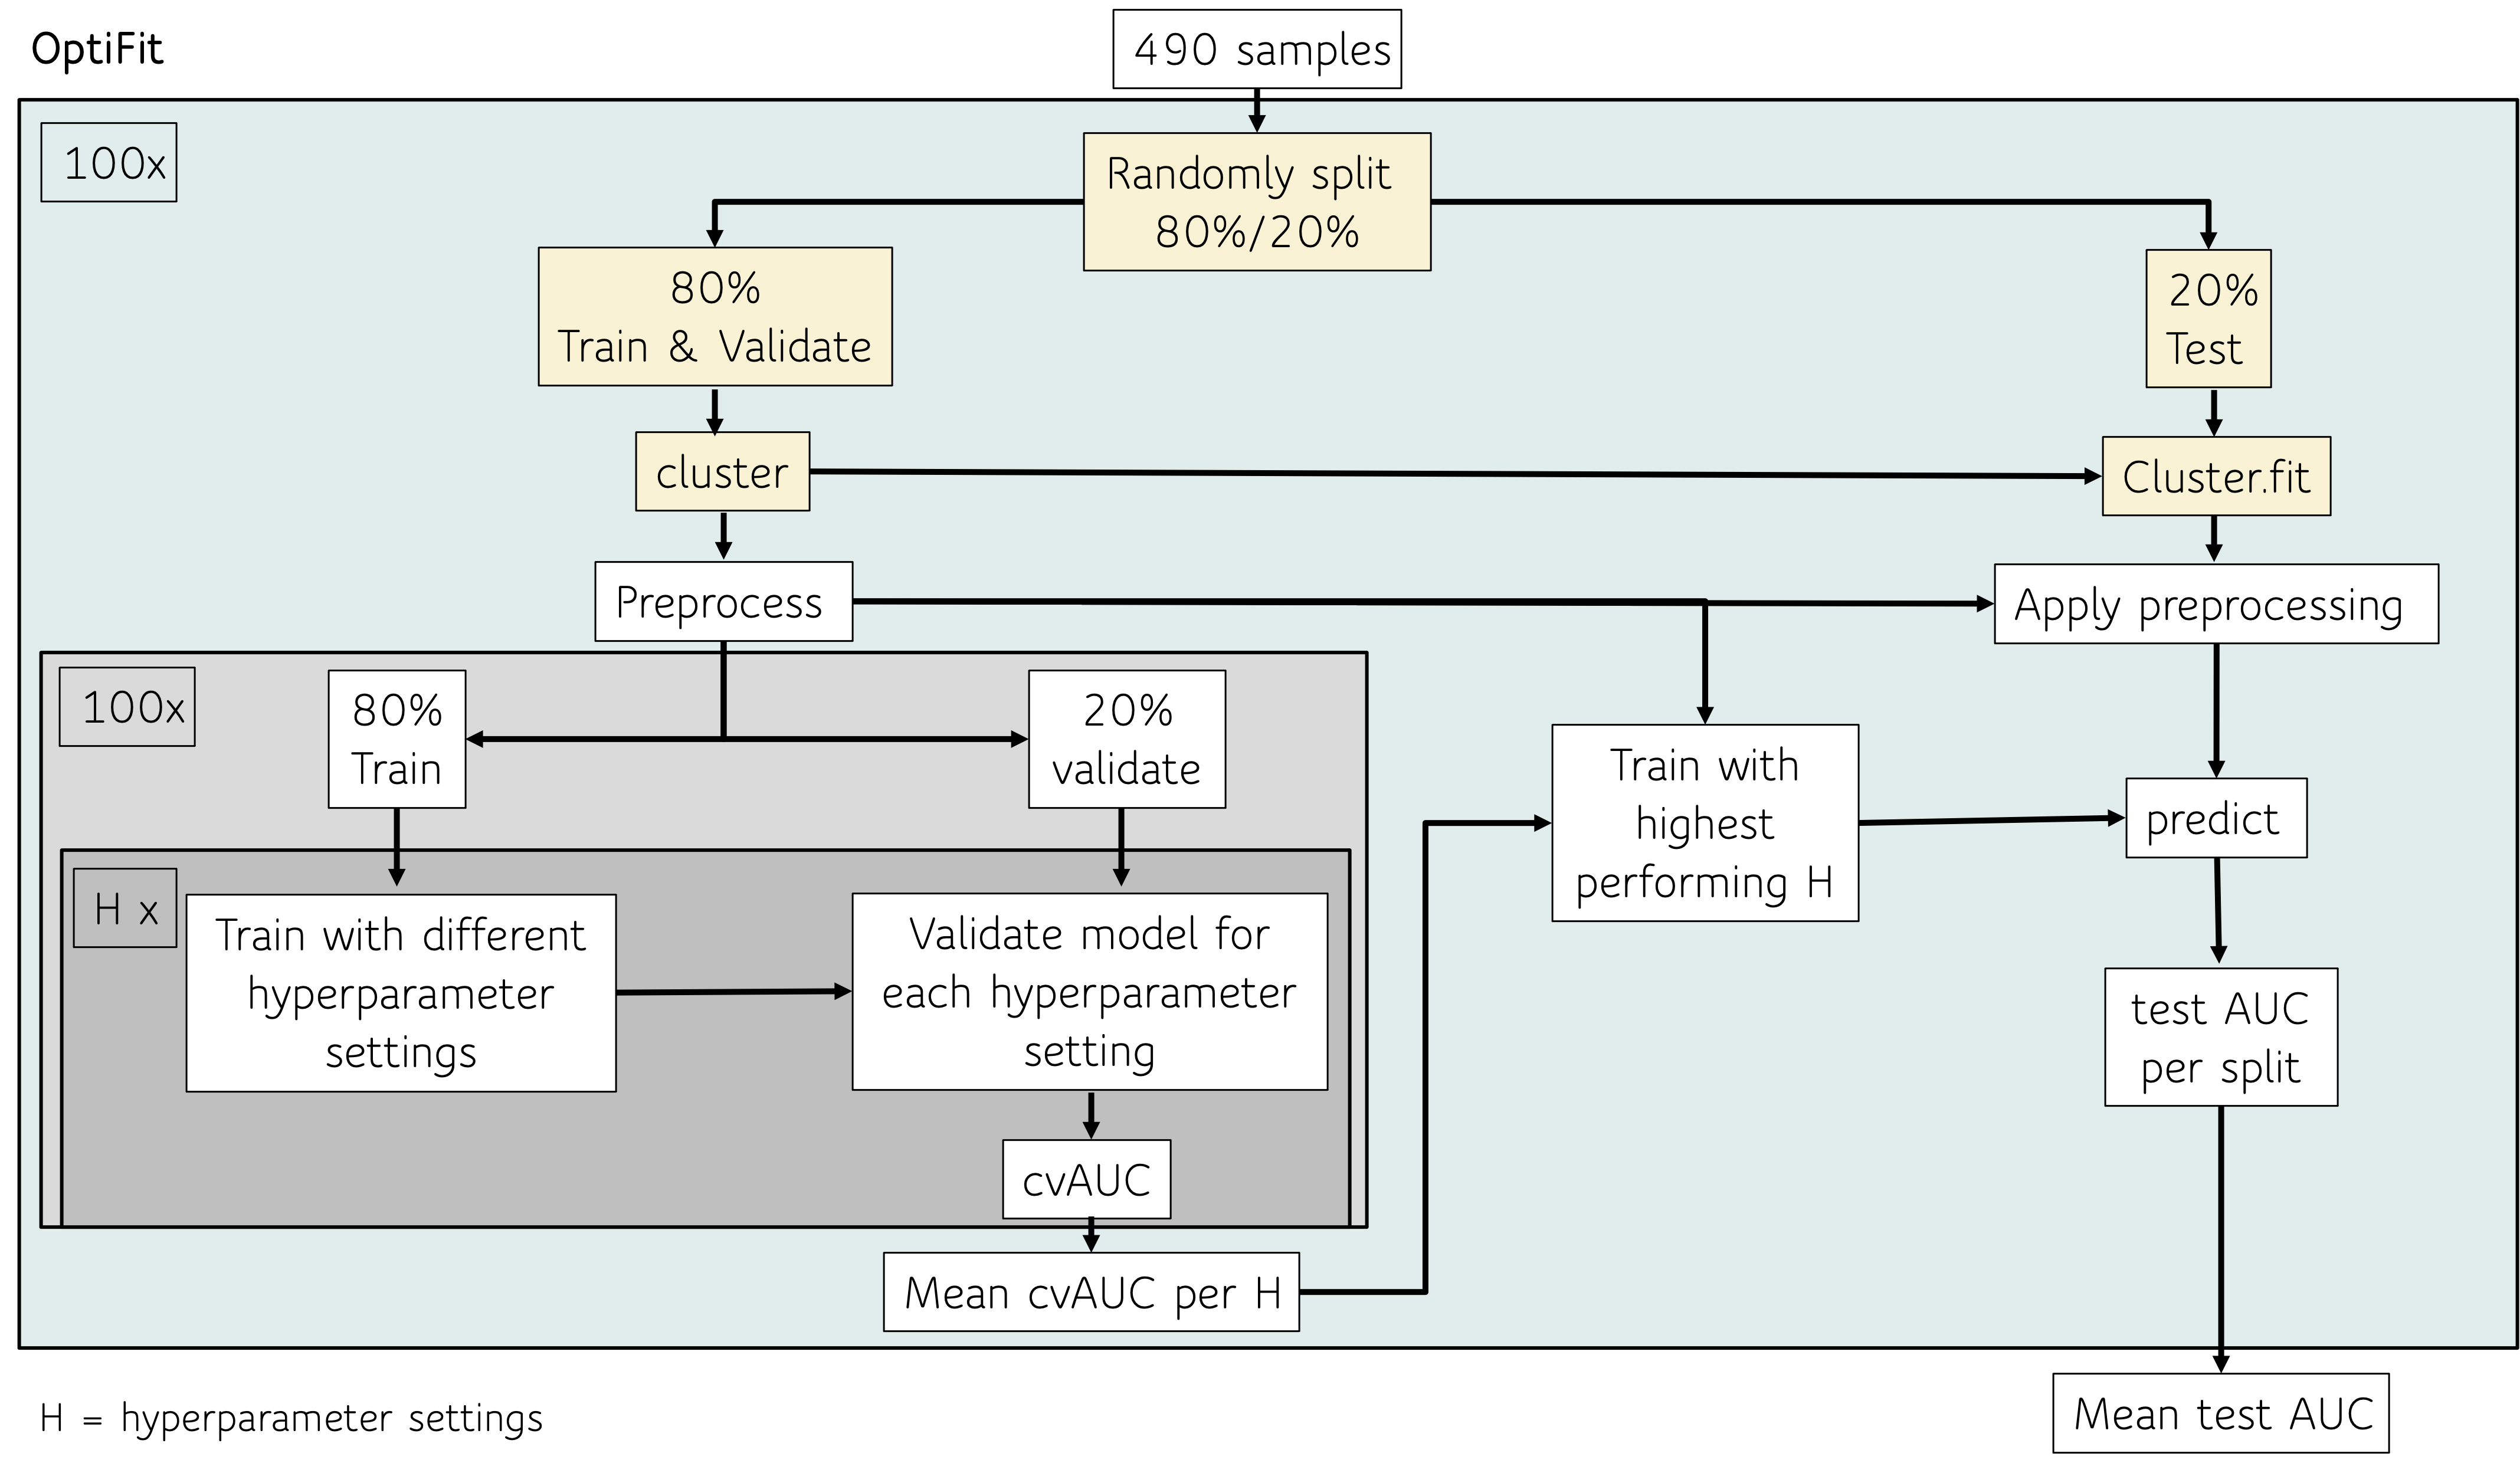
\includegraphics{../exploratory/figures/figure1B.png}
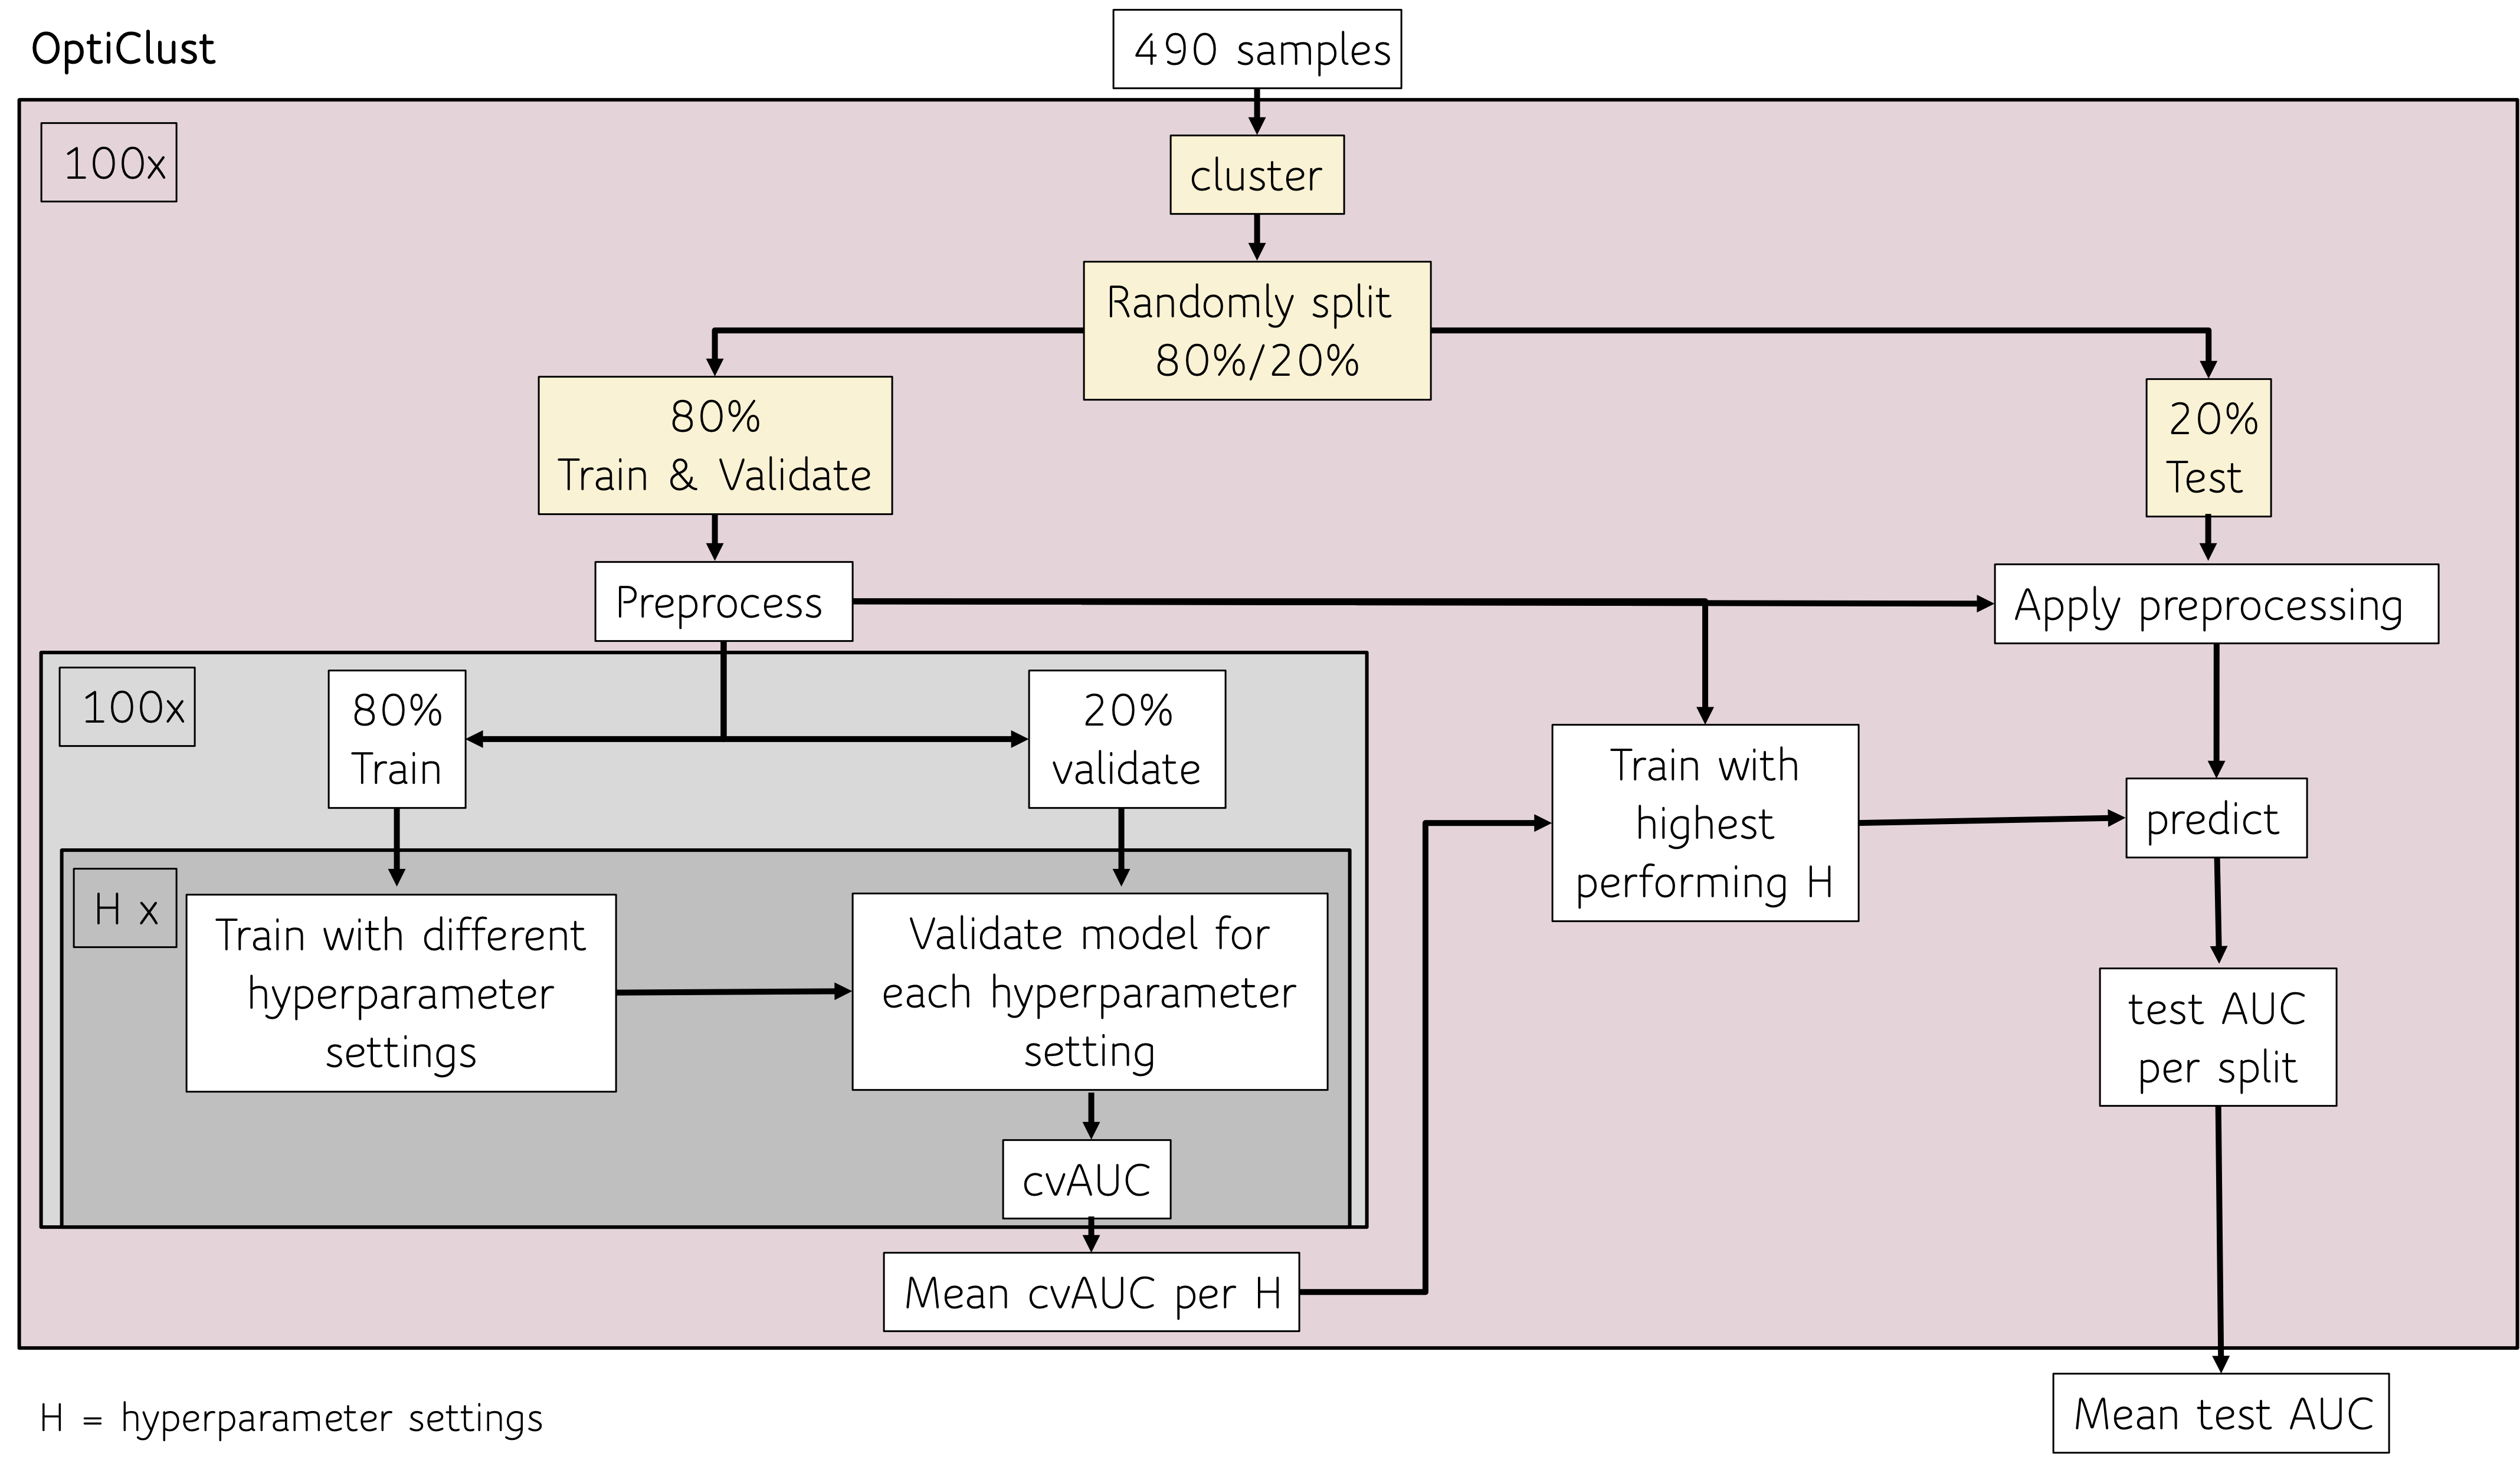
\includegraphics{../exploratory/figures/figure1Apng.png}

\textbf{Figure 1. Workflow} description.

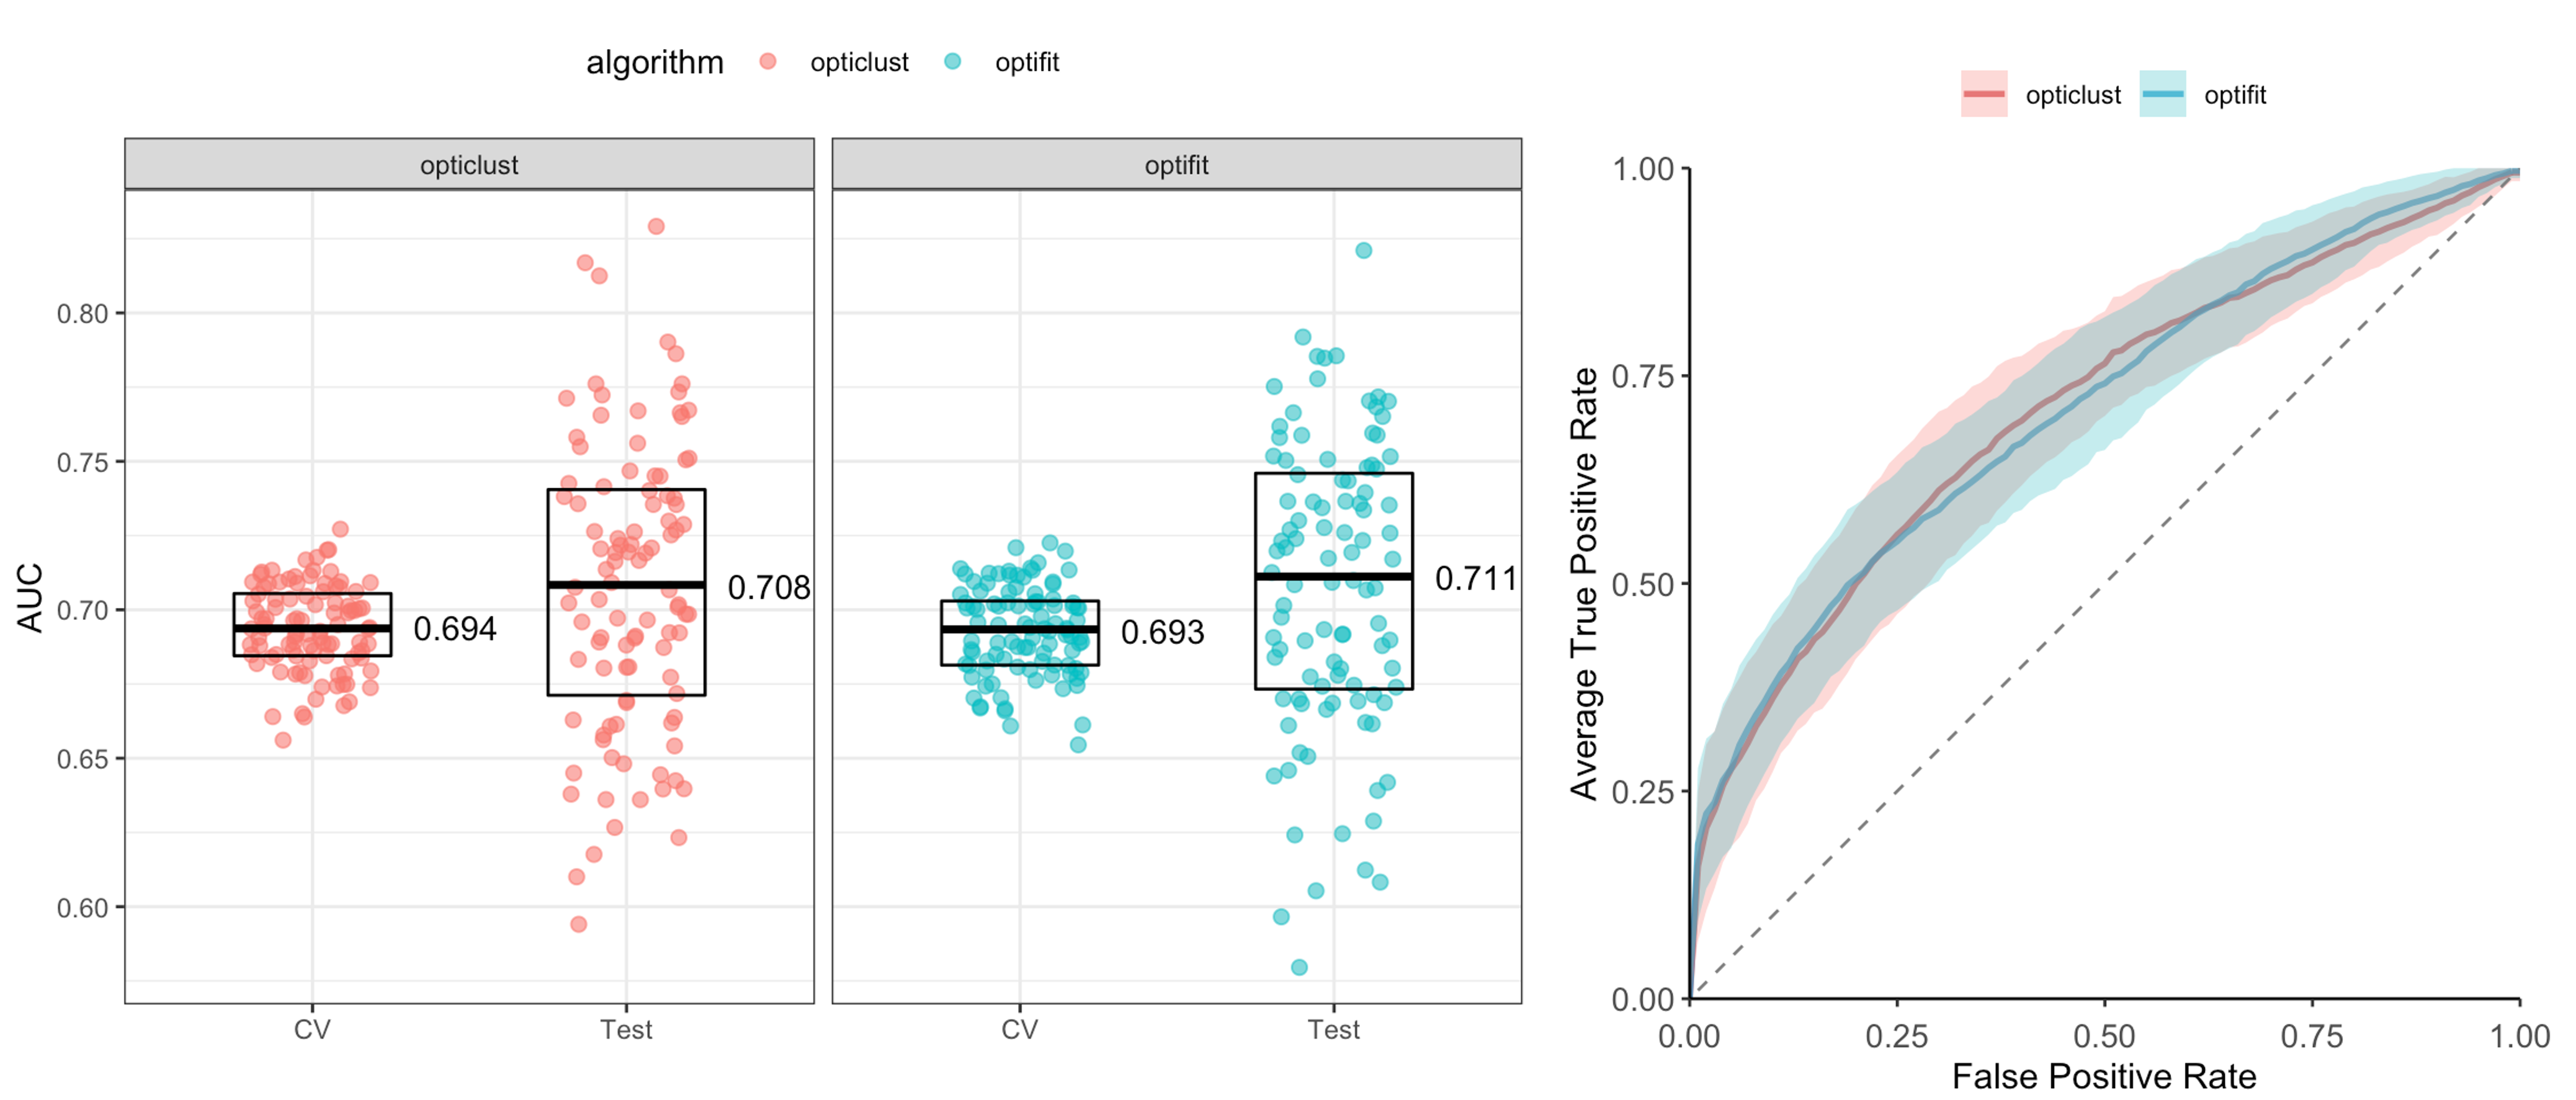
\includegraphics{../exploratory/figures/Figure2.png}

\textbf{Figure 2. Model Performance.} \textbf{A)} Mean AUC \textbf{B)}
Averaged ROC curves

\newpage

\hypertarget{references}{%
\subsection{References}\label{references}}

\end{document}
